\subsection{ASoC component controls}

\begin{frame}{\code{snd_soc_component_driver}}
  \begin{itemize}
  \item Controls allow to export configuration knobs of the component
    to userspace.
  \item ASoC provides many helpers to define them instead of filling
    \kstruct{snd_kcontrol_new}
  \end{itemize}
\end{frame}

\begin{frame}[fragile]{\code{snd_kcontrol_new}}
  \begin{block}{\kfile{include/sound/control.h}}
    \fontsize{9}{9}\selectfont
    \begin{minted}{c}
struct snd_kcontrol_new {
        snd_ctl_elem_iface_t iface;      /* interface identifier */
        unsigned int device;             /* device/client number */
        unsigned int subdevice;          /* subdevice (substream) number */
        const char *name;                /* ASCII name of item */
        unsigned int index;              /* index of item */
        unsigned int access;             /* access rights */
        unsigned int count;              /* count of same elements */
        snd_kcontrol_info_t *info;
        snd_kcontrol_get_t *get;
        snd_kcontrol_put_t *put;
        union {
                snd_kcontrol_tlv_rw_t *c;
                const unsigned int *p;
        } tlv;
        unsigned long private_value;
};
    \end{minted}
  \end{block}
\end{frame}

\begin{frame}[fragile]{kcontrol helpers}
  \begin{block}{\kfile{include/sound/soc.h}}
    \fontsize{9}{9}\selectfont
    \begin{minted}{c}
#define SOC_SINGLE(xname, reg, shift, max, invert) \
{       .iface = SNDRV_CTL_ELEM_IFACE_MIXER, .name = xname, \
        .info = snd_soc_info_volsw, .get = snd_soc_get_volsw,\
        .put = snd_soc_put_volsw, \
        .private_value = SOC_SINGLE_VALUE(reg, shift, max, invert, 0) }
#define SOC_SINGLE_RANGE(xname, xreg, xshift, xmin, xmax, xinvert) \
{       .iface = SNDRV_CTL_ELEM_IFACE_MIXER, .name = (xname),\
        .info = snd_soc_info_volsw_range, .get = snd_soc_get_volsw_range, \
        .put = snd_soc_put_volsw_range, \
        .private_value = (unsigned long)&(struct soc_mixer_control) \
                {.reg = xreg, .rreg = xreg, .shift = xshift, \
                 .rshift = xshift,  .min = xmin, .max = xmax, \
                 .invert = xinvert} }
#define SOC_SINGLE_TLV(xname, reg, shift, max, invert, tlv_array) \
{       .iface = SNDRV_CTL_ELEM_IFACE_MIXER, .name = xname, \
        .access = SNDRV_CTL_ELEM_ACCESS_TLV_READ |\
                 SNDRV_CTL_ELEM_ACCESS_READWRITE,\
        .tlv.p = (tlv_array), \
        .info = snd_soc_info_volsw, .get = snd_soc_get_volsw,\
        .put = snd_soc_put_volsw, \
        .private_value = SOC_SINGLE_VALUE(reg, shift, max, invert, 0) }
    \end{minted}
  \end{block}
\end{frame}

\begin{frame}[fragile]{kcontrol examples}
  \begin{block}{\kfile{sound/soc/codecs/pcm3168a.h}}
    \fontsize{9}{9}\selectfont
    \begin{minted}{c}
#define PCM3168A_DAC_PWR_MST_FMT                0x41
#define PCM3168A_DAC_PSMDA_SHIFT                7
    \end{minted}
  \end{block}
  \begin{block}{\kfile{sound/soc/codecs/pcm3168a.c}}
    \fontsize{9}{9}\selectfont
    \begin{minted}{c}
        SOC_SINGLE("DAC Power-Save Switch", PCM3168A_DAC_PWR_MST_FMT,
                        PCM3168A_DAC_PSMDA_SHIFT, 1, 1),
    \end{minted}
  \end{block}
  \begin{itemize}
  \item This exposes a simple on/off switch named "DAC Power-Save
    Switch" for bit 7 in register 0x41.
  \end{itemize}
\end{frame}

\begin{frame}[fragile]{kcontrol examples}
  \begin{block}{\kfile{sound/soc/codecs/pcm3168a.h}}
    \fontsize{9}{9}\selectfont
    \begin{minted}{c}
#define PCM3168A_ADC_MUTE                        0x55
    \end{minted}
  \end{block}
  \begin{block}{\kfile{sound/soc/codecs/pcm3168a.c}}
    \fontsize{9}{9}\selectfont
    \begin{minted}{c}
        SOC_DOUBLE("ADC1 Mute Switch", PCM3168A_ADC_MUTE, 0, 1, 1, 0),
    \end{minted}
  \end{block}
  \begin{itemize}
  \item This exposes a Left/Right switch named "ADC1 Mute Switch" for
    bit 0 (left) and 1 (right) in register 0x55.
  \end{itemize}
\end{frame}


\begin{frame}[fragile]{kcontrol examples}
  \begin{block}{\kfile{sound/soc/codecs/sgtl5000.h}}
    \fontsize{9}{9}\selectfont
    \begin{minted}{c}
#define SGTL5000_DAP_MAIN_CHAN            0x0120
    \end{minted}
  \end{block}
  \begin{block}{\kfile{sound/soc/codecs/sgtl5000.c}}
    \fontsize{9}{9}\selectfont
    \begin{minted}{c}
/* tlv for DAP channels, 0% - 100% - 200% */
static const DECLARE_TLV_DB_SCALE(dap_volume, 0, 1, 0);
[...]
        SOC_SINGLE_TLV("DAP Main channel", SGTL5000_DAP_MAIN_CHAN,
        0, 0xffff, 0, dap_volume),
    \end{minted}
  \end{block}
  \begin{itemize}
  \item This a single volume control named "DAP Main channel".
    It is controlled by register 0x120 and can take values up to
    0xffff.
  \end{itemize}
  \begin{block}{\kfile{include/uapi/sound/tlv.h}}
    \fontsize{9}{9}\selectfont
    \begin{minted}{c}
#define SNDRV_CTL_TLVD_DECLARE_DB_SCALE(name, min, step, mute) \
    \end{minted}
  \end{block}
\end{frame}

\begin{frame}[fragile]{kcontrol examples}
  \begin{block}{\kfile{sound/soc/codecs/pcm3168a.h}}
    \fontsize{9}{9}\selectfont
    \begin{minted}{c}
#define PCM3168A_DAC_VOL_MASTER                    0x47
    \end{minted}
  \end{block}
  \begin{block}{\kfile{sound/soc/codecs/pcm3168a.c}}
    \fontsize{9}{9}\selectfont
    \begin{minted}{c}
/* -100db to 0db, register values 0-54 cause mute */
static const DECLARE_TLV_DB_SCALE(pcm3168a_dac_tlv, -10050, 50, 1);
[...]
        SOC_SINGLE_RANGE_TLV("Master Playback Volume",
                        PCM3168A_DAC_VOL_MASTER, 0, 54, 255, 0,
                        pcm3168a_dac_tlv),
    \end{minted}
  \end{block}
  \begin{itemize}
  \item This a single volume control named "Master Playback Volume".
    It is controlled by register 0x47 and can take values 54 to 255.
    The datasheet states that 0 to 54 is mute.
  \end{itemize}
\end{frame}

\begin{frame}[fragile]{kcontrol examples}
  \begin{block}{\kfile{sound/soc/codecs/pcm3168a.h}}
    \fontsize{9}{9}\selectfont
    \begin{minted}{c}
#define PCM3168A_DAC_VOL_CHAN_START                0x48
    \end{minted}
  \end{block}
  \begin{block}{\kfile{sound/soc/codecs/pcm3168a.c}}
    \fontsize{9}{9}\selectfont
    \begin{minted}{c}
/* -100db to 0db, register values 0-54 cause mute */
static const DECLARE_TLV_DB_SCALE(pcm3168a_dac_tlv, -10050, 50, 1);
[...]
        SOC_DOUBLE_R_RANGE_TLV("DAC1 Playback Volume",
                        PCM3168A_DAC_VOL_CHAN_START,
                        PCM3168A_DAC_VOL_CHAN_START + 1,
                        0, 54, 255, 0, pcm3168a_dac_tlv),
    \end{minted}
  \end{block}
  \begin{itemize}
  \item This a Left/Right volume control named "DAC1 Playback Volume".
    Left is controlled by register 0x48, right channel is in register
    0x49 and both can take values 54 to 255.
    The datasheet states that 0 to 54 is mute.
  \end{itemize}
\end{frame}

\begin{frame}[fragile]{kcontrol examples}
  \begin{block}{\kfile{sound/soc/codecs/pcm3168a.h}}
    \fontsize{9}{9}\selectfont
    \begin{minted}{c}
#define PCM3168A_DAC_ATT_DEMP_ZF                0x46
#define PCM3168A_DAC_DEMP_SHIFT                 4
    \end{minted}
  \end{block}
  \begin{block}{\kfile{sound/soc/codecs/pcm3168a.c}}
    \fontsize{9}{9}\selectfont
    \begin{minted}{c}
static const char *const pcm3168a_demp[] = {
                "Disabled", "48khz", "44.1khz", "32khz" };

static SOC_ENUM_SINGLE_DECL(pcm3168a_dac_demp, PCM3168A_DAC_ATT_DEMP_ZF,
                PCM3168A_DAC_DEMP_SHIFT, pcm3168a_demp);
[...]
        SOC_ENUM("DAC De-Emphasis", pcm3168a_dac_demp),
    \end{minted}
  \end{block}
  \begin{itemize}
  \item This creates a control named "DAC De-Emphasis". Allowing to
    choose between four different values.
    This is controlled in register 0x46, bits 4 and 5.
  \end{itemize}
\end{frame}

\begin{frame}[fragile]{kcontrol examples}
  \begin{block}{\kfile{sound/soc/codecs/sgtl5000.h}}
    \fontsize{9}{9}\selectfont
    \begin{minted}{c}
#define SGTL5000_DAP_AVC_THRESHOLD                0x0126
    \end{minted}
  \end{block}
  \begin{block}{\kfile{sound/soc/codecs/sgtl5000.c}}
    \fontsize{9}{9}\selectfont
    \begin{minted}{c}
static int avc_get_threshold(struct snd_kcontrol *kcontrol,
                             struct snd_ctl_elem_value *ucontrol)

[...]
static const DECLARE_TLV_DB_MINMAX(avc_threshold, 0, 9600);
[...]
        SOC_SINGLE_EXT_TLV("AVC Threshold Volume", SGTL5000_DAP_AVC_THRESHOLD,
                        0, 96, 0, avc_get_threshold, avc_put_threshold,
                        avc_threshold),
    \end{minted}
  \end{block}
  \begin{itemize}
  \item This a single volume control named "AVC Threshold Volume".
  \end{itemize}
\end{frame}

\begin{frame}{kcontrol names}
  \begin{itemize}
  \item Naming actually matters, userspace tools use them to populate
    the user interface properly!
  \item Controls named similarly will be grouped together:
    \begin{itemize}
    \item "Playback" and "Capture" controls may be exposed separately
      in the UI
    \item "Mute Switch" and "Volume" for a similarly named controls
      can be shown as a single control
    \end{itemize}
  \end{itemize}
  \vspace{1em}
  \begin{minipage}[b]{0.35\textwidth}
    \begin{itemize}
    \item Master Playback Switch
    \item Master Playback Volume
    \item Headphone Mic Boost Volume
    \item Capture Volume
    \end{itemize}
    \vfill~
  \end{minipage}
  \hfill
  \begin{minipage}[b]{0.62\textwidth}
    \centering
    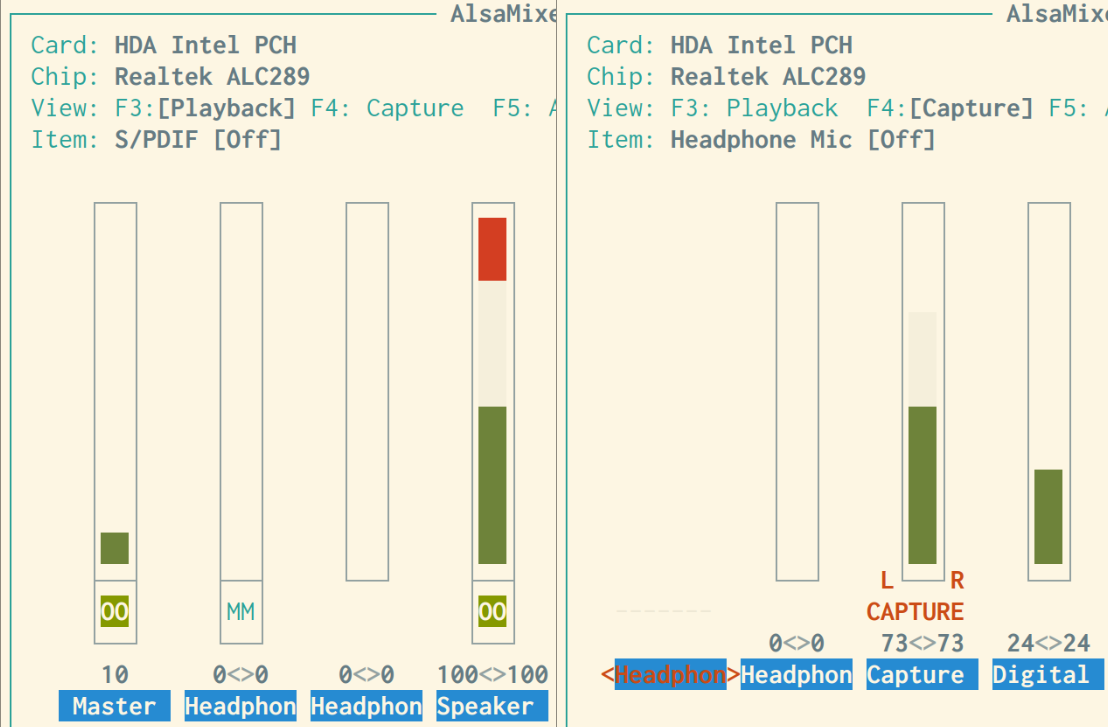
\includegraphics[width=.6\textwidth]{slides/audio-asoc-component-controls/alsamixer.png}
  \end{minipage}
  \begin{center}
  \end{center}
\end{frame}



